\section{Background}
\label{sec:background}

Un metodo efficace per l'astrazione del concetto consiste 
in una rappresentazione tramite un reticolo, in inglese ``lattice''.

% \begin{definition}[Reticolo]
%     Un reticolo è un insieme di punti (siti), ciascuno in grado di identificare un 
%     ordine locale per il riconoscimento dei primi vicini.
%     I siti sono collegati tra di loro tramite degli archi (legami), che 
%     possono esistere solo tra due primi vicini.
% \end{definition}

\begin{definition}[Reticolo]
    Un reticolo $L$ di dimensione $n$ è una coppia $\langle S, B \rangle$, dove:
    \begin{itemize}
        \item $S = \left\{ s_i : i \in \mathbb{N} , \, 0 \leq i < n \right\}$ è l'insieme dei siti;
        \item $B = \left\{ (s_i, s_j) \in S^2 \, : \text{$s_i$ e $s_j$ siano primi vicini} \right\}$ è 
        
        l'insieme dei legami.
    \end{itemize}
\end{definition}
Due siti possono essere considerati primi vicini se, secondo l'ordinamento locale dei siti, hanno 
distanza uguale a 1.
In un reticolo in cui vale questa relazione è possibile descrivere due tipi di percolazione: 
percolazione di sito e percolazione di legame.
% \begin{itemize}
%     \item percolazione di legame;
%     \item percolazione di sito.
% \end{itemize}

\begin{figure}
    \centering
    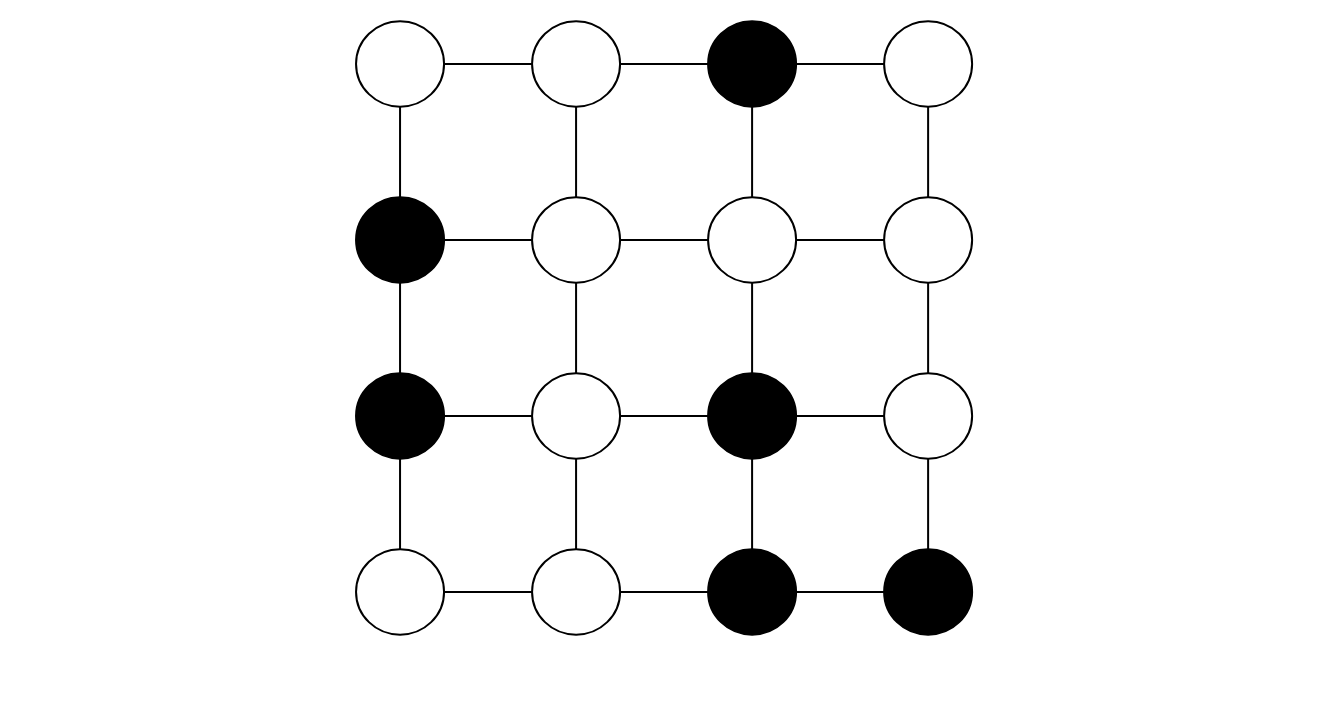
\includegraphics[width=0.4\textwidth]{2D-lattice}
    \caption{Esempio di reticolo quadrato bidimensionale}
    \label{fig:ex-lattice}
\end{figure}

\subsection*{Percolazione di legame}
È la prima versione del modello fornita da Broadbent e Hammersley \cite{broadbent}.
Ogni legame ha probabilità $p$ di essere ``aperto'', quindi
probabilità $1-p$ di essere ``chiuso''. Se due siti formano un legame aperto, vi è una
connessione diretta tra i due. Al contrario, un legame chiuso elimina la connessione.
In questa versione, ``avviene percolazione'' se esiste un percorso (insieme di connessioni dirette) 
che attraversa l'intero reticolo. La percolazione può verificarsi 
sia in verticale (alto-basso) sia in orizzontale (sinistra-destra).

\subsection*{Percolazione di sito}
In questo modello ogni sito ha una probabilità $p$ di essere occupato, di conseguenza
probabilità $1-p$ di essere vuoto. In figura \ref{fig:ex-lattice} viene mostrato un 
reticolo bidimensionale quadrato con nodi occupati (neri) e vuoti (bianchi). Questo è 
il modello che verrà utilizzato per lo studio dell'argomento e dei vari algoritmi e verrà
approfondito in dettaglio nella sezione \ref{sec:implementazione}.

\subsection*{Soglia di percolazione}
I due modelli appena introdotti rappresentano soluzioni valide per lo studio 
del fenomeno. Nonostante la somiglianza, vi sono differenze concettuali che si 
riflettono anche nel calcolo di alcuni valori caratteristici \cite{weisstein-bond,weisstein-site,weisstein-threshold}.

\begin{definition}[Soglia di percolazione]
    Sia $L$ un reticolo di dimensione infinita\footnote{Con il termine ``infinito'' 
    si fa riferimento all'estensione intuitiva delle varie proprietà della struttura,
    come avviene in matematica per il concetto di \textit{limite all'infinito}.}. 
    Sia $p$ la probabilità di occupazione di un sito o di apertura 
    di un legame, a seconda del modello scelto. 
    Sia $p$ uguale per ogni elemento del reticolo.
    La soglia di percolazione per $L$ è definita come la 
    probabilità $p_c$ tale per cui:
    \begin{itemize}
        \item se $p > p_c$, allora vi è percolazione;
        \item se $p < p_c$, allora non vi è percolazione.
    \end{itemize}
\end{definition}

\begin{figure}
    \centering
    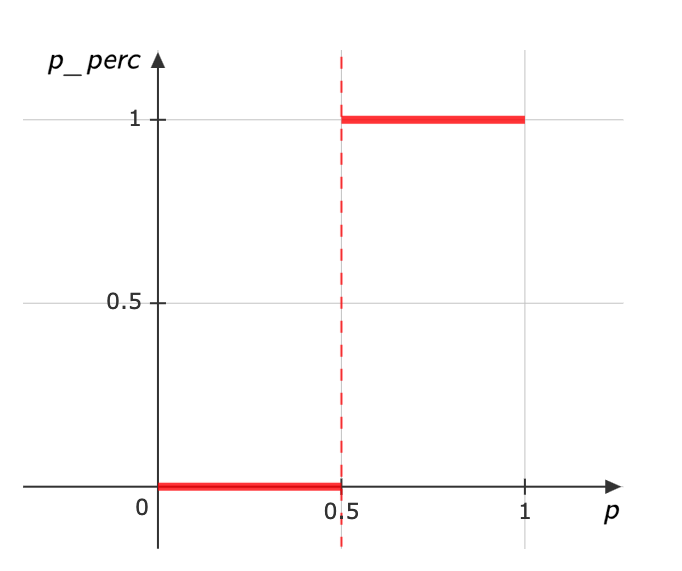
\includegraphics[width=0.4\textwidth]{threshold.png}
    \caption{Grafico relativo alla soglia di percolazione ($p_c=0.5$)}
    \label{fig:threshold}
\end{figure}

È possibile visualizzare il concetto di soglia nel grafico mostrato in 
figura \ref{fig:threshold}, in cui l'asse delle ascisse è associato alla 
probabilità $p$, mentre l'asse delle ordinate è associato alla probabilità
che avvenga percolazione $p_{perc}$.

Nei casi reali, ovvero per reticoli di taglia finita, non è possibile stabilire
un'affermazione così forte. 
Ciò che è possibile preservare dalla definizione 
è che esiste un \textbf{punto critico} $p_c$ relativo alla probabilità $p$, oltre 
al quale è più probabile che avvenga percolazione e, al contrario, al di sotto
del quale è meno probabile che questo si verifichi.

\begin{table}[ht!]
    \centering
    \begin{tabular}{lcc}
    \toprule
    \textbf{Lattice} & \textbf{\(p_c\) (Site)} & \textbf{\(p_c\) (Bond)} \\
    \midrule
    Cubic (body-centered) & 0.246    & 0.1803    \\
    Cubic (face-centered) & 0.198    & 0.119     \\
    Cubic (simple)        & 0.3116   & 0.2488    \\
    Diamond               & 0.43     & 0.388     \\
    Honeycomb             & 0.6962   & 0.65271*  \\
    4-Hypercubic          & 0.197    & 0.1601    \\
    5-Hypercubic          & 0.141    & 0.1182    \\
    6-Hypercubic          & 0.107    & 0.0942    \\
    7-Hypercubic          & 0.089    & 0.0787    \\
    Square                & 0.592746 & 0.50000*  \\
    Triangular            & 0.50000* & 0.34729*  \\
    \bottomrule
    \end{tabular}
    \caption{Punti critici (\(p_c\)) per reticoli regolari.}
    \label{tab:percolation}
\end{table}

In letteratura sono presenti diversi studi sulle caratteristiche di vari 
reticoli e i rispettivi valori di soglia. La tabella \ref{tab:percolation}
mostra i punti critici per diversi reticoli regolari, ovvero composti
da elementi ripetuti della stessa forma. La colonna \textbf{Lattice} indica la forma 
del reticolo, mentre le colonne \textbf{Site} e \textbf{Bond} distinguono i valori 
in percolazione di sito e di legame, rispettivamente \cite{stauffer-threshold}.
Vi è una lieve, ma evidente, discrepanza tra i valori nelle due colonne.
In generale, la rappresentazione tramite occupazione dei siti è considerata
più generica rispetto alla sua controparte, questo perché la percolazione di legame
può essere riformulata in termini di percolazione di sito, 
ma non si può affermare il contrario.
I valori affiancati da un asterisco possono essere trovati tramite calcoli analitici,
grazie ad alcune caratteristiche della forma del reticolo,
sono quindi considerati \textit{conosciuti}. È interessante notare che la 
tabella è composta per lo più da valori non conosciuti, cioè valori ottenuti da 
simulazioni al calcolatore.

\subsection*{Cluster-finding}
Nel modello che opera sui siti, la percolazione viene rilevata in seguito a un processo 
di \textit{cluster-finding}, che consiste nel partizionare il reticolo in diverse 
classi, tramite una relazione di equivalenza. 
\begin{definition}
Una relazione di equivalenza $R$ su un insieme $A$ è una relazione binaria 
che gode delle seguenti proprietà:
\begin{itemize}
    \item $\forall x \in A : xRx$ (riflessività);
    \item $\forall x,y \in A : xRy \rightarrow yRx$ (simmetria);
    \item $\forall x,y,z \in A: xRy \wedge yRz \rightarrow xRz$ (transitività).
\end{itemize}
\end{definition}
La relazione utilizzata è strettamente collegata al concetto di primi vicini.
La definizione di primi vicini per un sito può variare a seconda della tipologia
(forma e dimensioni) del reticolo utilizzato.

\subsection*{Distribuzione binomiale}
Per formalizzare in modo completo il modello, è necessario introdurre 
la nozione di \textit{variabile aleatoria}. Non verrà trattato l'argomento 
nel dettaglio, per lasciare più spazio alle implementazioni.
In questo contesto, si introduce il concetto di variabile aleatoria come 
una variabile il cui valore dipende da un evento non deterministico.
Questo evento è descritto attraverso funzioni di densità specifiche, che seguono 
leggi di \textit{distribuzione} della probabilità \cite{random}. Esistono diverse 
tipologie di distribuzioni, tra cui quella binomiale che, riassumendo, descrive 
un esperimento di prove ripetute.
Questo tipo di distribuzione è caratterizzato da una funzione di densità 
a 2 parametri
\begin{equation}
    \mathcal{B}_{n, p}(k) = \binom{n}{k} p^k (1-p)^{n-k}
\end{equation}
\label{eq:binom}
dove $n$ rappresenta il numero di prove e $p$ la probabilità di successo di ciascuna.
La variabile $k$ indica il risultato di cui vogliamo verificare la probabilità.
L'equazione \ref{eq:binom} rappresenta \textit{`` la probabilità che si ottengano $k$ successi
ripetendo $n$ volte una prova con probabilità di successo $p$ ''}.

\subsection{Distribuzione Gaussiana}
La distribuzione normale o gaussiana è una delle distribuzioni di probabilità più importanti 
in statistica e probabilità. La sua funzione di densità probabilistica (PDF) è data da:
\begin{equation}
    f(x) = \frac{1}{\sigma \sqrt{2\pi}} e^{-\frac{(x - \mu)^2}{2 \sigma^2}}, \quad x \in \mathbb{R},
\end{equation}
dove $\mu$ rappresenta la media e $\sigma^2$ la varianza.
Questa distribuzione emerge naturalmente in numerosi contesti scientifici e 
tecnici grazie al \textit{Teorema del Limite Centrale}.

\subsection{Legge dei Grandi Numeri in forma di Chebyshev}
La \textit{Legge dei Grandi Numeri} afferma che la media aritmetica di una sequenza di variabili aleatorie indipendenti
 e identicamente distribuite (iid) converge alla loro media attesa quando il numero di osservazioni tende all'infinito. 
 Una formulazione basata sulla disuguaglianza di Chebyshev è la seguente:
\begin{equation}
    P\left( \left| \frac{1}{n} \sum_{i=1}^{n} X_i - \mathbb{E}[X] \right| \geq \epsilon \right) \leq \frac{\text{Var}(X)}{n \epsilon^2}, \quad \forall \epsilon > 0,
\end{equation}
dove $X_i$ sono variabili aleatorie iid
con media finita $\mathbb{E}[X]$ e varianza finita $\text{Var}(X)$.
 Questo implica che all'aumentare di $n$, la probabilità che la media campionaria si discosti dalla media 
 attesa oltre una certa soglia si riduce.

\subsection{Teorema del Limite Centrale}
Uno dei risultati fondamentali della teoria della probabilità è il \textit{Teorema del Limite Centrale} (TLC), 
il quale afferma che, date $X_1, X_2, \dots, X_n$ variabili aleatorie indipendenti e identicamente distribuite 
con media $\mu$ e varianza finita $\sigma^2$, la variabile normalizzata:
\begin{equation}
    Z_n = \frac{\sum_{i=1}^{n} X_i - n\mu}{\sigma \sqrt{n}}
\end{equation}
converge in distribuzione a una variabile casuale normale standard $\mathcal{N}(0,1)$ per $n \to \infty$:
\begin{equation}
    Z_n \sim \mathcal{N}(0,1).
\end{equation}
Questo risultato giustifica l'uso della distribuzione normale in molte applicazioni pratiche, in particolare nella statistica inferenziale e nella teoria dell'approssimazione.